\documentclass[11pt]{report}
\listfiles

\usepackage[margin=2.5cm]{geometry}
\usepackage[colorlinks]{hyperref}
 \usepackage{glossaries} % acronym will go in main glossary
 %\usepackage[acronym]{glossaries} % make a separate list of acronyms

\makeglossaries
\usepackage{graphicx}
\setcounter{secnumdepth}{5}
\setcounter{tocdepth}{5}
\begin{document}

\begin{titlepage}

\begin{center}


% Upper part of the page

\includegraphics[scale=1.0]{images/logo.png}

\textsc{\LARGE University of Western Ontario}\\[1.5cm]

\textsc{\Large Software Specifications: Camera Simulation Environment}\\[0.5cm]


% Title
{ \huge \bfseries Version 0.02}\\[0.4cm]

% Author and supervisor
\begin{minipage}{0.4\textwidth}
\begin{flushleft} \large
\emph{Author:}\\
Kartik \textsc{Thakore} \\
kthakore@uwo.ca 
\end{flushleft}
\end{minipage}
\begin{minipage}{0.4\textwidth}
\begin{flushright} \large
\emph{Supervisors:} \\
Dr.~Hanif \textsc{Ladak}\\
Dr.~Terry \textsc{Peters} 
\end{flushright}
\end{minipage}

\vfill

% Bottom of the page
{\large \today}

\end{center}

\end{titlepage}
\bibliographystyle{IEEE}
\nocite{*}

\tableofcontents

\listoffigures 

\printglossaries

\newpage 

\chapter{Revisions}
\begin{center}
\begin{tabular}{| l | c | l | p{9cm} |}
\hline
Date & Version & Author & Description \\ 
\hline
January 22 2012 & 0.01 & Kartik Thakore & Initial Specifications Document \\
\hline
Feburary 1 2012 & 0.02 & Karitk Thakore & Incorporating Dr. Ladak's Changes \\
\hline
\end{tabular}
\end{center}

\chapter{Introduction}
  
A core component of Medical Imaging application is the use of computer vision. Camera calibration is a common task required for computer vision. Camera calibration can be a difficult task for researchers without prior graphics background. Cameras have been modeled extensively in literature, and thus can be simulated. A virtual environment provides an activity based learning approach for camera calibration. 
     
\section{Overview}

\newacronym[\glsshortpluralkey=VR]{VR}{VR}{Virtual Reality: is a simulated environment that is implemented to provide a simulated experience of a real world process or activity}

\newglossaryentry{extrinsic}{name={extrinsic},
description={Parameters of a camera that define the coordinte system transformations from 3D world coordinates to 3D camera coordinates. Two matrices are provided \(R\) and \(T\) }}
  \newglossaryentry{intrinsic}{name={intrinsic},
description={A single matrix that contains 5 parameters. The parameters incorporate focal length, image format and principal point. }}
  
\begin{enumerate}
\item A virtual reality (\glsname{VR}) environment that simulates \glsname{extrinsic} and \glsname{intrinsic} parameters of a camera will provide a sufficient model to allow training on transformation matrices involved with camera calibration.
\item Camera calibration of a simple camera system, performed with prior training in a virtual reality environment, will yield insignificantly different capture camera parameters with real world camera system. 
\end{enumerate}

\section{Background and Significance}

Medical Imaging tasks such as image fusion, registration, feature tracking, etc. are built on the understanding of the mathematical concepts of vision systems. Computer vision is an increasing component of image-guided interventions. Moreover it is often difficult for researchers not from a computer vision background to learn quickly. Virtual environments that simulate computer vision systems will both hasten the learning curve and also act as a prototyping environment for new applications of video-based technology in image-guided interventions. 

\newglossaryentry{pcm}{name={Pinhole Camera Model},
description={The pinhole camera model defines a camera as a mathematical relation between the coordinates of a 3D point, projected onto an image plane. This is also called the Perspective Model. It is a common camera model used in computer vision}}


Mathematically, vision systems can be represented as matrices that perform operations on a spatial field. Cameras in medical imaging essentially transform three-dimensional content to two-dimensional planes (\gls{pcm} \cite{CV}). Thus, locations in 2D images correspond to the position and orientation of objects in the real world.

To be able to capture the position and orientation of objects, a transformation matrix is required from the 2D images. This transformation matrix is acquired by performing camera calibration. Calibration involves acquiring images of known objects with known positions and orientations in the real space. Next, feature points are selected on the 2D image. The selection of feature points are done either manually or using libraries such as OpenCV. The correspondence sets up the transformation between the real world coordinate system and the image coordinates.

Simulation of this process can begin by modeling the camera using the perspective projection model. The model can be represented in matrix notation as:

\begin{equation} s * \mathbf{p} = \mathbf{A} * [\mathbf{R}|\mathbf{t}] * \mathbf{P}  \end{equation}
 
where  \(A\) is defined as the \glsname{intrinsic} matrix, \(s\) represents the arbitrary scale factor, \(p\) are the 2D image coordinates, \(P\) are the corresponding 3D world coordinates, and finally \((R|t)\) are the \glsname{extrinsic} parameters.

The \glsname{intrinsic} matrix can be calculated from camera dependent parameters such as focal length and CCD pixel. Additionally, the \glsname{extrinsic} parameters are user defined such that rotation and translation are selected by the user. Finally, the \(P\) world coordinates are simply defined by the user and the scene that will rendered in the virtual reality environment. 

A key challenge faced by graduate students in areas such as image-assisted surgery is in learning the calibration process and understanding the sensitivity of the calibration results on estimated parameters. Indeed, experience at the Robart's Research Institute indicates that students can take several months to learn about camera calibration. Simulation will allow for applications such as training and prototyping. 

\newglossaryentry{SIT}{name={SIT},
description={SIT: System Integration Testing, tests the overall system via, given inputs and expected outputs}}

\newglossaryentry{UAT}{name={UAT},
description={UAT: User Acceptance Testing, tests the system to ensure the user experience and expectations are met}}

Once the prototype software system is developed, System Integration Testing (\glsname{SIT}) will be performed. Validation will be performed with User Acceptance Testing (\glsname{UAT}) of a selected group of volunteers. This will aid in narrowing down the causes for difficulty with understanding camera calibration. 

\section{Relevance}

Camera calibration is a difficult task and a widely recurrent task at Robart's Research Institute in Medical Imaging. Additional camera calibration is a means to an end in most projects and not the focus. The essential tasks involved for performing a camera calibration are similar across projects with potential for standardization and collaboration. In Dr. Peters' laboratory, a considerable amount of effort is placed in camera calibration in several research projects. Each project involves isolated or loosely collaborated work on camera calibration. No software currently exists to help with training of camera collaboration. 

Selecting a camera is crucial to a medical imaging application. A virtual environment may help to explore and compare various camera systems based on parameters provided by manufacturers. Allowing researchers to objectively try systems rather then purchasing each system and performing manual calibration. This will facilitate prototyping and will be a boon for researchers in  gaining an intuitive understanding into the critical factors of camera calibration and the impact on their application. 

\section{Scope}
The scope of this project is primarily to create a virtual environment that can reasonably simulate common cameras used in medical applications. The system will be able to create cameras given parameters that can be used to view a scene and run camera calibration tests on. Once calibrated, the system will allow the user to capture virtual images. 
 
\begin{enumerate}
\item Develop a \glsname{VR} environment that can calculate transformation matrices based on given locations, poses, and camera parameters.  
\item Implement a \glsname{VR} environment that simulates camera calibration within user specified scenes. Develop an online tool that can be accessed by a wide audience in the medical imaging field.
\end{enumerate}

\subsection{Pilot Scope}
The scope of this pilot is to explore and define (from the prespective of a new researcher) more deeply the problems with camera calibration, and a possible solution.  

\section{Technical Overview}

\subsection{User Interface}

\newglossaryentry{webb}{name={Web Browser},
description={A cross platform software package to view HTTP provided content from service providers}}

\newglossaryentry{Javascript}{name={Javascript},
description={A cross platform scripting language that runs on the client side}}

\newglossaryentry{HTML5}{name={HTML5}, description={Is the fifth version of the Hypertext Markup Language that provides many new features such as canvas and web sockets}}
\newglossaryentry{WebGL}{name={WebGL}, description={A web technology being developed by the Khronos Group to bring accelerated graphics to the web browser}}

One of the initial aims of this project was to provide a easily distributed user interface. A web interface is a proven technology in providing distributed interfaces. The user interface provided by this system will be designed on a \glsname{HTML5}/\glsname{WebGL} project that will work over pre-specified \glsname{webb}. \glsname{WebGL} sits on top of \glsname{HTML5}'s canvas feature and will provide 3D rendering capabilities on enabled \glsname{webb}. Most user demographics are familiar with using a \glsname{webb}, which makes this an ideal option. 

\glsname{WebGL} will be written in the \glsname{Javascript} language that is a platform provided by most modern \glsname{webb}. 

The \glsname{webb} is also very portable compared to other solutions, as most modern computer systems come with one installed. The need to have a \glsname{WebGL} enabled \glsname{webb} may hinder the proliferation of the system. However most new versions of \glsname{webb} are coming with \glsname{WebGL} enabled and it is a emerging trend.

The \glsname{webb} finally also comes at no additional cost to the user.  

An alternative option involves creating custom distribution and front end software ( similar to a \glsname{webb} ). This is not feasible with the time frame for a Masters project.  

\subsection{Application Server}

\newglossaryentry{app}{name={Application Server},
description={A web service provider that responds to requests from the client}}

An \glsname{app} will be built to provide the \glsname{Javascript} and \glsname{HTML5} documents to the \glsname{webb}. Additionally, the server will utilize middleware platforms that help to scale (ensures the \glsname{app} responds to requests from multiple \glsname{webb}s).

\subsubsection{HTTP Server}

\newglossaryentry{HTTP}{name={HTTP}, description={ HyperText Transport Protocol defines the protocol of transporting documents to a web client}}

The \glsname{HTTP} Server will be responsible for responding to requests sent by \glsname{webb} clients. The key requirement required of the \glsname{HTTP} Server is to scale reasonably with an increase in demands. Most of the computational expense will be done on the \glsname{webb} client, due to the way \glsname{WebGL} works. A scalable \glsname{HTTP} Server will ensure that the response for the \glsname{WebGL} and \glsname{HTML5} documents are provided in a timely manner. For this reason the Nginx \glsname{HTTP} Server and a Starman/PSGI middleware server will be used.

A middleware server allows multiple \glsname{app} to be initiated and used in parallel for times of load. This facilitates the reliability and scalability of the system. 

\subsubsection{Dispatch/Controller}

\newglossaryentry{OpenCV}{name={OpenCV}, description={A software library that has a camera calibration component}}

The user will be using the system to do camera calibration that will require a interface between the frontend and \glsname{OpenCV} features. A controller will be used to define to protocol by which the frontend will communicate with the \glsname{OpenCV} Server. 

\subsubsection{OpenCV Server}

This server will provide the \glsname{app} with \glsname{OpenCV} features such as camera calibration and re-projection of calibration grids.

\chapter{User Specifications}

This chapter defines the user of this system and their specifications. Defining the user ensure that the system can be designed with a \glsname{UAT} goal in mind. 

\begin{figure}[htp]
\centering
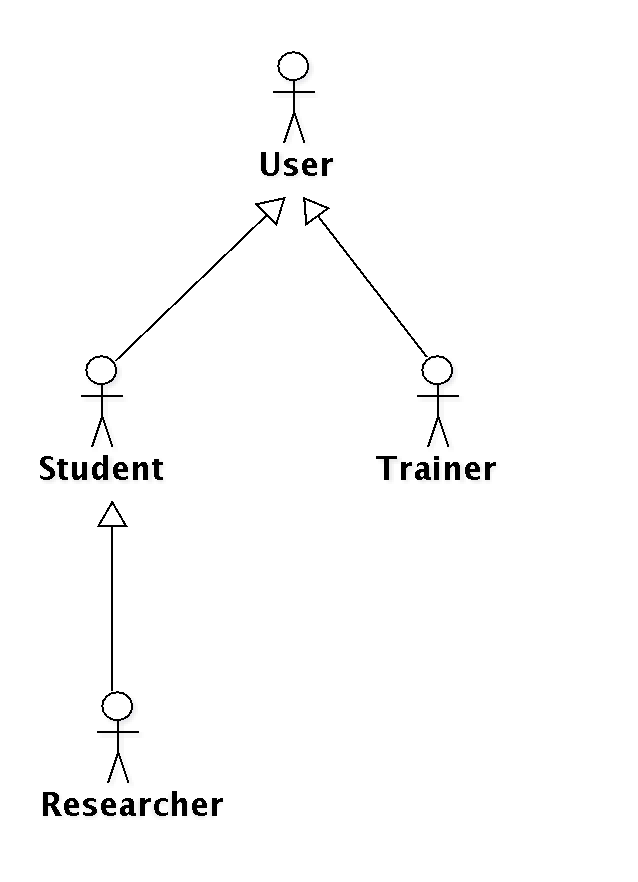
\includegraphics[scale=0.25]{images/UserOverview.png}
\caption{Users}
\label{fig:uo}
\end{figure}

\section{Users} 

The system user is a generalization of several other users as depicted in the use case diagram \ref{fig:uo}.  

\subsection{Student}

The student user is the primary user of the system. This system is essentially made to facilitate the understanding of the student user. Student users are defined as any user that needs to learn and work with camera transformation.  

\subsubsection{Researcher}

The student user can also be extended as a researcher who needs a deeper understanding of camera calibration for a research project. These project involve camera calibration as a critical component in the implementation. 

\subsection{Trainer}

Another user that may use the system is the trainer. Trainer users use the system as a guide for students and researchers. The direct requirements of the trainer user needs to be captured at a later date.

\section{Use Cases}

Use Cases define the process the system will take to meet the needs of the users. Each use case is written in a list format showing what the user will see and react with during the specific portion of the system. 
\subsubsection{Camera Calibration}

\begin{figure}[htp]
\centering
\includegraphics[scale=0.40]{images/AllUserCases.png}
\caption{Generic User Cases}
\label{fig:guc}
\end{figure}


As described in \ref{fig:guc}, users can perform the camera calibration procedure as defined in Chapter 2 of \cite{CC}. All users of the system can perform a camera calibration procedure. 

The first step involves creating a camera by with specified measurements. Users in future versions may select existing cameras that have been validated and stored on the system. 


\begin{figure}[htp]
\centering
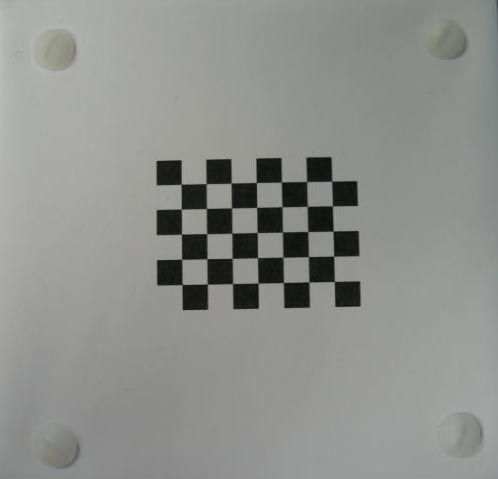
\includegraphics[scale=0.45]{images/board.png}
\caption{Calibration Grid --\cite{CC}}
\label{fig:grid}
\end{figure}

Using the camera the User can then select an origin point and place calibration grids ( shown in figure \ref{fig:grid} ) within the \glsname{VR}. The user then capture the placement of the calibration grids as images.
The images are analyzed for lens distortion (provided by \glsname{OpenCV}). 


\begin{figure}[htp]
\centering
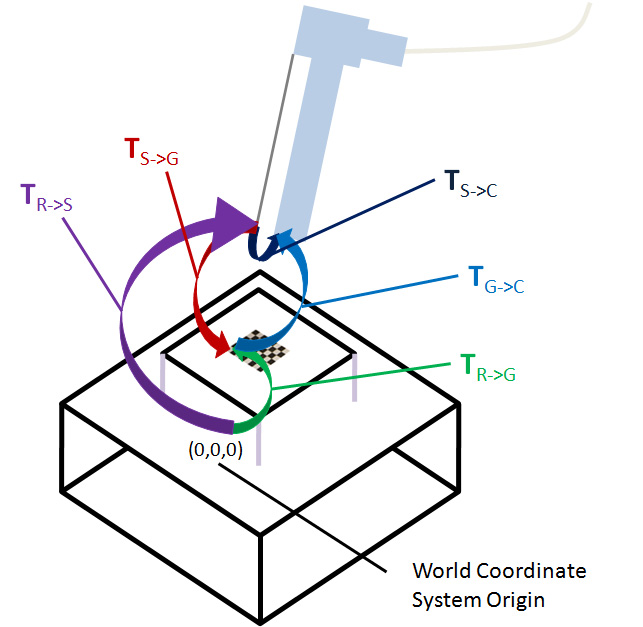
\includegraphics[scale=0.45]{images/Coordinates.png}
\caption{Transformations involved during Calibration --\cite{CC}}
\label{fig:coord}
\end{figure}

\subsubsection{Constructing Transforms}
The user can apply the camera calibration by mapping the calibrated camera's origin point to a real world coordinate system.  Further analysis of the use case is required to decide between a haptic arm or mouse solution.

This transforms between the calibrated transforms and the real world application (depicted by \( T_{R->S} \) in \ref{fig:coord} ). Finally by adjusting the lens distortion parameters the user can compare the accuracy at real world points between sets of distortion parameters.  

\subsubsection{Comparing Camera Systems} 

\begin{figure}[htp]
\centering
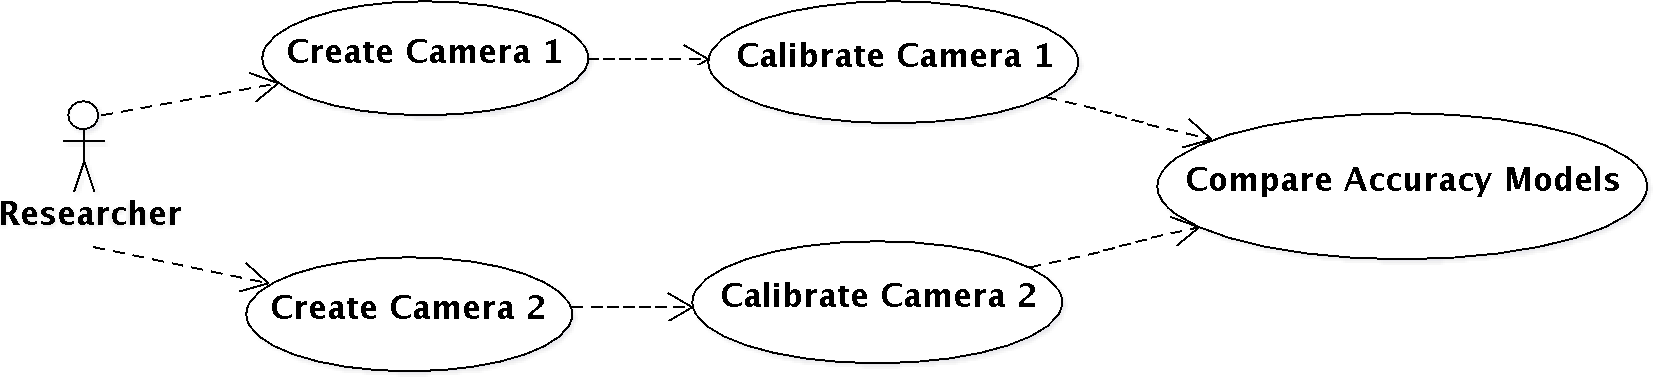
\includegraphics[scale=0.15]{images/CompareCameras.png}
\caption{Researcher Use Cases}
\label{fig:ucc}
\end{figure}

The Researcher user can perform calibration on two cameras and compare their accuracy models, to decided if they are suitable for their application. This use case is depicted in figure \ref{fig:ucc}.

\subsubsection{Training}

\begin{figure}[htp]
\centering
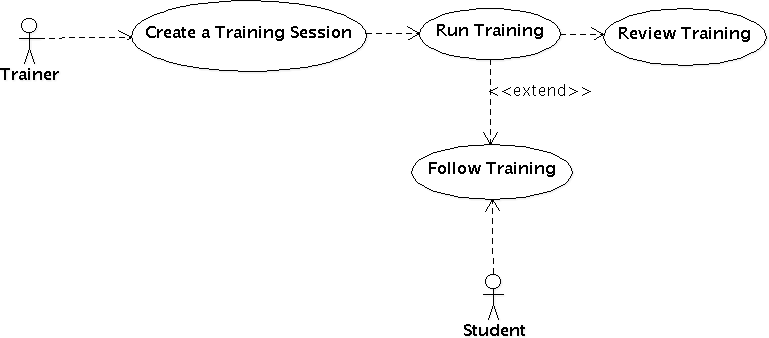
\includegraphics[scale=0.45]{images/Training.png}
\caption{Generic Training User Cases}
\label{fig:uco}
\end{figure}

Training involves two users. The Trainer can create a training session with a specified calibration procedure (camera, distortions, grid ... etc). Then the Trainer can send this session to a Student. 

The Student will follow the Training Session and work towards a specified goal by the Trainer. The Student can also leave their feedback on completion that the Trainer can review, as described on \ref{fig:uco}

The Student completes the training session by finishing camera calibration and sending back the camera distortion parameters, \glsname{extrinsic} and \glsname{intrinsic} values to the trainer. Additionally the student can record the difficulty level of the steps of camera calibration. This feedback can be reviewed by the trainer.  


\chapter{System Requirement Specifications}

\newglossaryentry{SRS}{name={SRS}, description={Software/System Requirement Specifications}}


The follow System Requirement Specifications (\glsname{SRS}) serve to outline a set of deliverables or goals for the prototyping period of analysis, design, and implementation. The preliminary specifications are defined here to provide a starting point for prototyping. The initial round of testing on the prototype will help to clarify, extend and solidify the next iteration of specifications. This document is meant to modified and iterated.  

\section{User Interface} 

The user interface will be designed with standard \glsname{HTML5} provided components for capturing user inputs, and providing feedback. These elements are well known and understood by a wide variety of users, reducing the steepness of the learning curve.

\subsection{Interface Overview}

There are no specific requirements for the user interface as of yet; however a general understanding of the screens has been captured as described in \ref{fig:is}. 

\begin{figure}[htp]
\centering
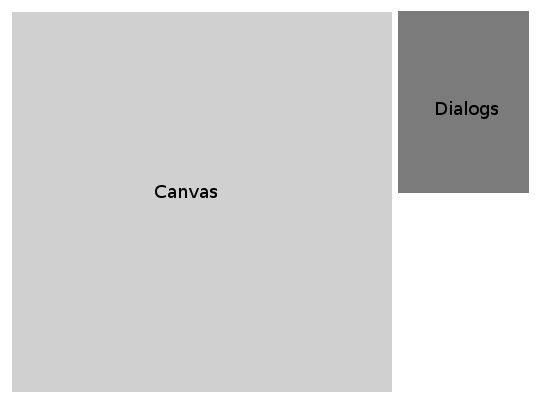
\includegraphics[scale=0.45]{images/interface_screen.png}
\caption{Interface Overview}
\label{fig:is}
\end{figure}

The interface overview can be broken down into two sections. The canvas and the options menu. All 'work' related with camera calibration will be visualized in the canvas section of the interface. All inputs will be captured in the dialogs section of the interface. Any additional outputs will be show via the dialogs sections also.

\subsubsection{Canvas}

The canvas will be a \glsname{WebGL} environment which which visualize the 3D state of the client. 

\section{Data Models}

The data models of the system are software constructs that the client holds, containing groups of related data. The models may or may not be sent to the \glsname{app} for storage. 

\subsection{Storage}

Models will be stored as a JSON (Javascript Object Notation) within the \glsname{Javascript} cache of the client. Client side storage will be temporary and non persistent per user session.

\subsection{Known Models}

The current known models are:

\subsubsection{Camera}

Attributes include:

\begin{enumerate}
\item name: human readable content to allow comparison.
\item measurements: measured values as described in the use case \ref{fig:guc}
\item calibration session: status of the current calibration procedure. Including the \glsname{extrinsic}, \glsname{intrinsic} and distortion values.  
\end{enumerate}

\subsubsection{Calibration Session}

Attributes include:
\begin{enumerate}
\item name: human readable content to allow comparison.
\item steps: predetermine step in calibration. This will be a generic template, until various procedures are designed by a Trainer.
\item matrices: \glsname{extrinsic}, \glsname{intrinsic} and distortion values 
\item coordinates system: coordinate systems associated with this calibration 
\end{enumerate}

\subsubsection{Training Session}

Attributes include: 
\begin{enumerate}
\item camera: camera to work with (specified by Trainer) 
\item student: name of the student currently working on the calibration, including email.
\item calibration feedback: comments of the student and difficulty  
\item trainer: email of the trainer 
\end{enumerate}

\subsubsection{Student Feedback}

Attributes include: 
\begin{enumerate}
\item difficulty: rating 
\item description: written comments 
\end{enumerate}

\section{Functional Requirements}

\subsection{Create Camera}

User will complete the Camera data model described earlier. 

\subsection{Calibration}

User will select a calibration grid and pose it 6 times within the 3D canvas. 
User will use an \glsname{OpenCV} interface to retrieve distortion parameters.
User will analyse and derive the \glsname{extrinsic} and \glsname{intrinsic} values of the parameters. 

\subsection{Accuracy Modeling}

\newglossaryentry{Frustum}{name={Frustum}, description={Viewing volume of a camera}}

\begin{figure}[htp]
\centering
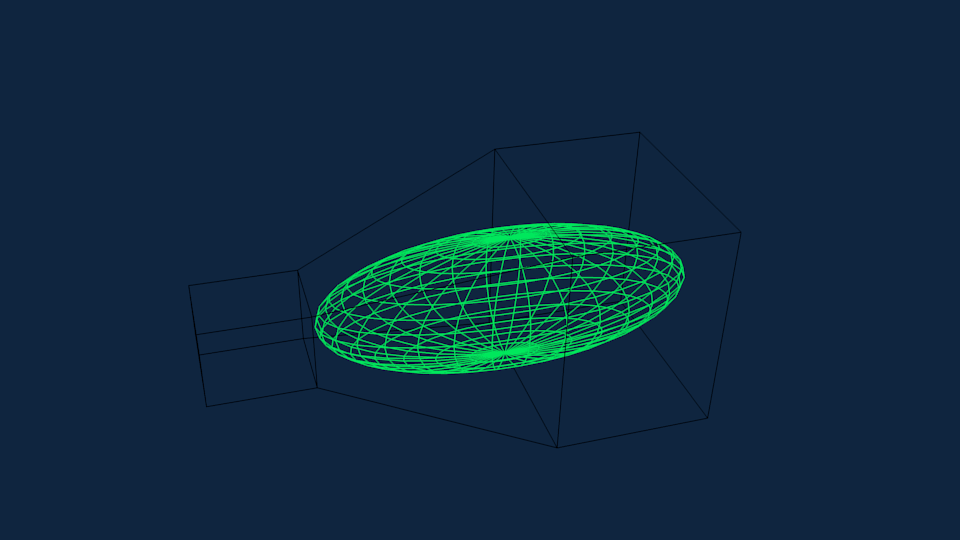
\includegraphics[scale=0.50]{images/accuracy_vizulization.png}
\caption{Visualising the accuracy model within the frustum of a Camera }
\label{fig:av}
\end{figure}


User will adjust distortion project and project the selected calibration grids to selected poses. System will calculate difference between points on the actual and projected grid. 
The accuracy can also be taken with placing points within the viewing range (\glsname{Frustum}) of each camera and calculating difference between ideal (no distortions) and changing distortions. 

User can also perform accuracy modeling between two cameras to decide which one to pick. The accuracy will be visualized to show areas of acceptable accuracy that the user picks. A potential visualization concept is depicted in the figure \ref{fig:av}. 


\subsection{Training} 

The Trainer will provide a student's email, and decide on steps for training on (changes in data models). The steps are created to watch for changes in the data models(such as values confirmed for \glsname{extrinsic} matrix). These are essentially steps that can be watched and associated with student's tasks within the larger activity of camera calibration. 

The trainer can then send a hyper text link via email to the student. The student  will go to the link and follow the training steps while providing the feedback. The feedback will collect the student's difficulty and provide a report to the trainer. 

The trainer can then review each step and then work with the Student to eliminate learning problems within identified difficult areas.  

\section{Constraints}

\subsection{Reliability}

Reliability constraints are the same as expected of other web tools available. Industry standards of scalability are deployed into the system. Further testing will need to be performed to ensure expected reliability. This will be performed in \glsname{UAT}.  

\subsection{Scalability}

Scalability constraints are the same as expected of other web tools available. Industry standards of scalability are deployed into the system. 

\subsection{Performance}

Performance constraints are lax, as this is a prototype and performance profiles are not available. 

\subsection{Security} 

Currently there are no security constraints known. 


\bibliography{software_specs}{}

\end{document}
